\chapter{Resultados Experimentais} \label{chap:resexp}


Os testes desta secção têm como objetivo encontrar o melhor detetor / descritor / matcher , determinando a robustez do subsistema de localização para o ruído, iluminação variante e rotação.

Os parâmetros utilizados nos vários detetores para limitar o número de pontos característicos são definidos com base no valor médio de intensidade da imagem. Desta forma, os detetores trabalham sob várias condições de brilho.

Para obter resultados constantes, a plataforma ROS permite ao usuário reproduzir uma sequência de mensagens nas mesmas condições em que foram adquiridas. Esta funcionalidade permite ao desenvolvedor resultados constantes, ou seja, diferentes combinações de parâmetros podem ser testadas para a mesma entrada exata.

\section{Calibração da câmara}

Como mencionado anteirormente, no capítulo ~\ref{section:Intrin}, as câmara e lente têm que ser calibrada para não causar erros de distorção nos resultados finais. 

\begin{figure}[h!]  %colocar figura a seguir ao texto anterior
	\centering
	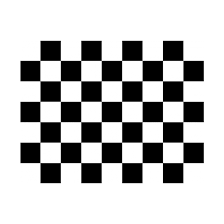
\includegraphics[width=0.4\linewidth]{checkboard.png} 
	\caption{Quadrado de xadrez para calibrar câmara.}
	\label{fig:checkboard}  %30 years. Figure 3 a)
\end{figure}

Desta forma, é usado o algoritmo desenvolvido em ~\cite{piCam}. O algoritmo baseia-se no uso de um quadrado de xadrez , figura ~\ref{fig:checkboard}. Este é composto por quadrados com a mesma largura e devido à sua composição em xadrez é fácil a determinação de pontos de intreseção \ cruzamento. Com estes pontos é possivel criar linhas com tamanhos conhecidos e através destas obter os parâmetros intrinsecos da camâra e lente. 



A figura ~\ref{fig:imgcheckboard} ilustra a calibração da devida câmara do raspberry pi com uma lente olho de peixe \textit{full-frame}. O resultado final é a matriz de parâmetros intrinsecos composta por : \[ \left[ \begin{array}{ccc}
603.104 & 0 & 651.767 \\ 
0 & 601.316 & 337.810 \\ 
0 & 0 & 1
\end{array} \right] \] e matriz de parâmetros de distorção \[ \left[\begin{array}{ccccc}
-0.308 & 0.0729 & 0.00208 & -0.00157 & 0 
\end{array} \right] \]

\begin{figure}[h!]  %colocar figura a seguir ao texto anterior
	\centering
	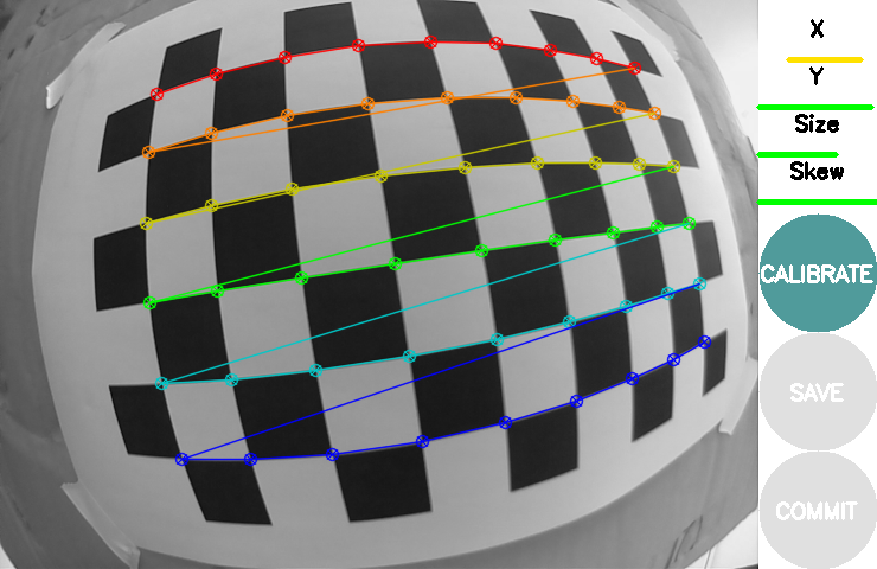
\includegraphics[width=0.6\linewidth]{imgcheckboard.png} 
	\caption{Imagem da calibração dos parâmetros da câmara.}
	\label{fig:imgcheckboard}  %30 years. Figure 3 a)
\end{figure}


Desta forma, é possível retirar a distorção de uma imagem lente olho de peixe . 



Como ilustrado na figura ~\ref{fig:FishEyeN} a imagem possui a distorção de lente olho de peixe e um grnade ângulo de abertura. Removida a distorção da imagem é obtida a figura ~\ref{fig:FishEyeUndist} na qual é reduzido o ângulo de abertura.

\begin{figure}[h!]
	\centering
	\subfloat[\label{fig:FishEyeN}]{
		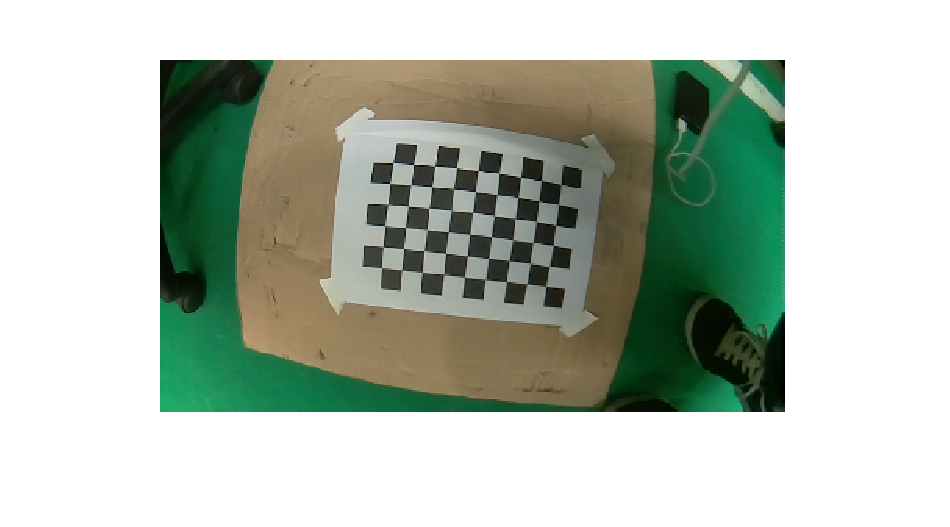
\includegraphics[width=0.4\textwidth]{ImagemFishEye.eps}}
	\qquad
	\subfloat[\label{fig:FishEyeUndist}]{
		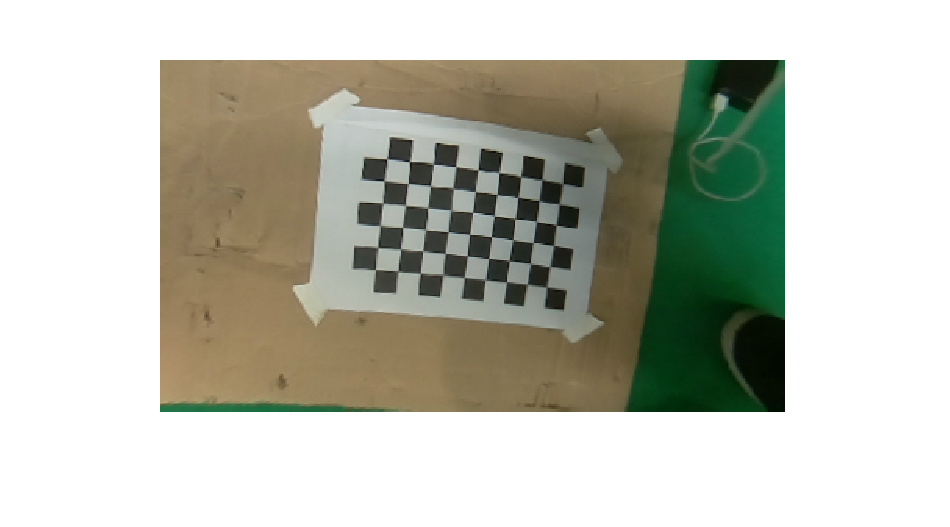
\includegraphics[width=0.4\textwidth]{ImagemFishEyeUndist.eps}}
	\caption{Diferença entre ângulos de abertura em imagem com e sem distorção.}\label{fig:FisheEye}
\end{figure}


Quando removido a distorção da imagem o ângulo de abertura diminui mas continua sendo maior que o ângulo de uma camara sem lente olho de peixe, como ilustrado na figura ~\ref{fig:ImageNorm}. Esta foi capturada com a mesma camara sem lente olho de peixe e à mesma distância do quadrado de xadrez.

\begin{figure}[h!]
	\centering
	\label{fig:ImageNorm}
	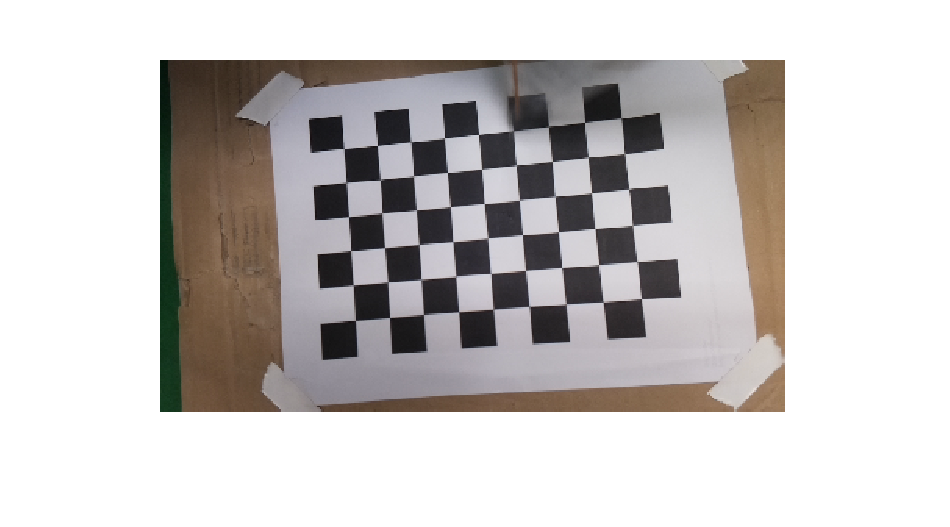
\includegraphics[width=0.4\textwidth]{ImagemNormal.eps}
	\caption{Imagem sem lente olho de peixe.}
\end{figure}







\section{Diferença entre detetores de características}

Nesta dissertação serão comparados 4 detetores de características, explicitos em  ~\ref{detCar}. Os testes são realizados num ambiente agrícola para maior coerência com o objectivo da dissertação, como ilustrado na figura ~\ref{fig:metodosALL}.


%\begin{figure}[h!]  %colocar figura a seguir ao texto anterior
%	\begin{center}
%	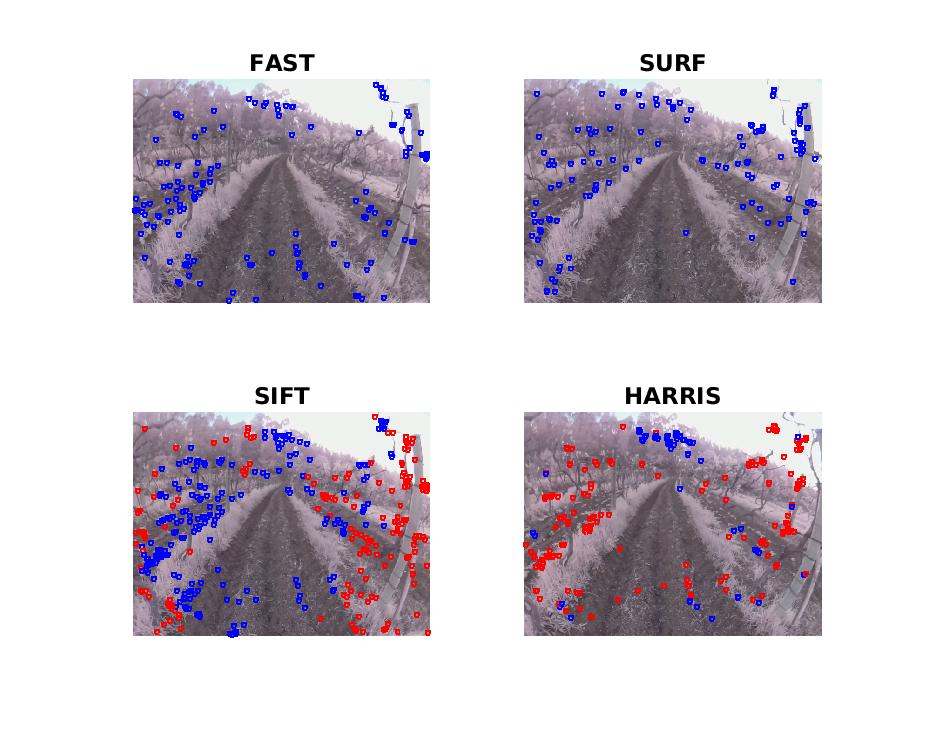
\includegraphics[width=0.8\linewidth]{FAST_SURF_SIFT_HARRIS.eps} 
%	\caption{Distribuição dos pontos caracterisiticos para os quatro detetores de características, FAST , SURF, SIFT, HARRIS.}
%	\label{fig:4metodos}  %30 years. Figure 3 a)
%	\end{center}
%\end{figure}


\begin{figure}[h!]
	\centering
	\subfloat[FAST\label{fig:metodosFAST}.]{
		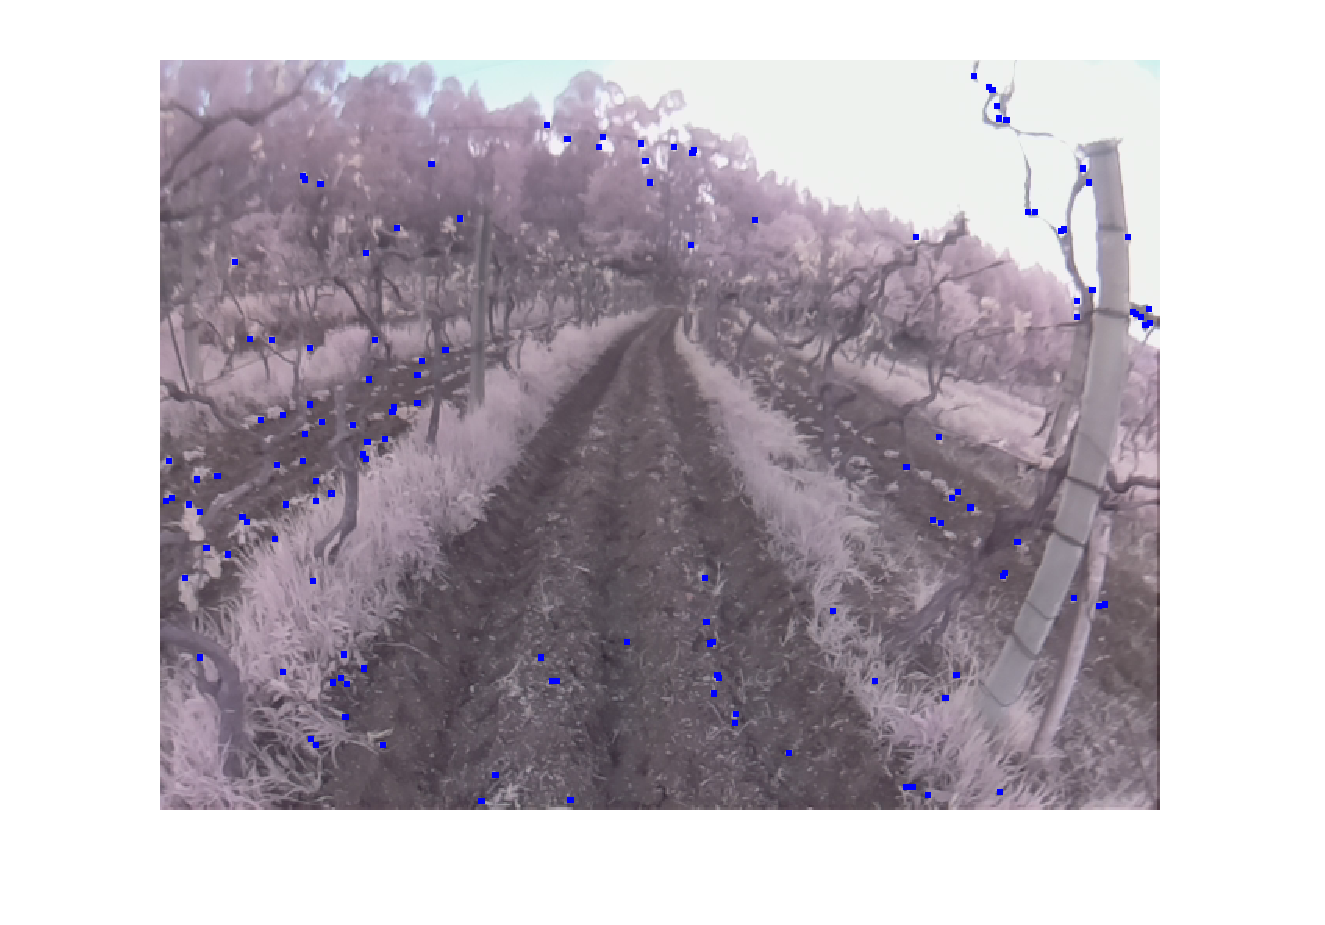
\includegraphics[width=0.4\textwidth]{metodosFAST.eps}}
	\qquad
	\subfloat[SURF\label{fig:metodosSURF}.]{
		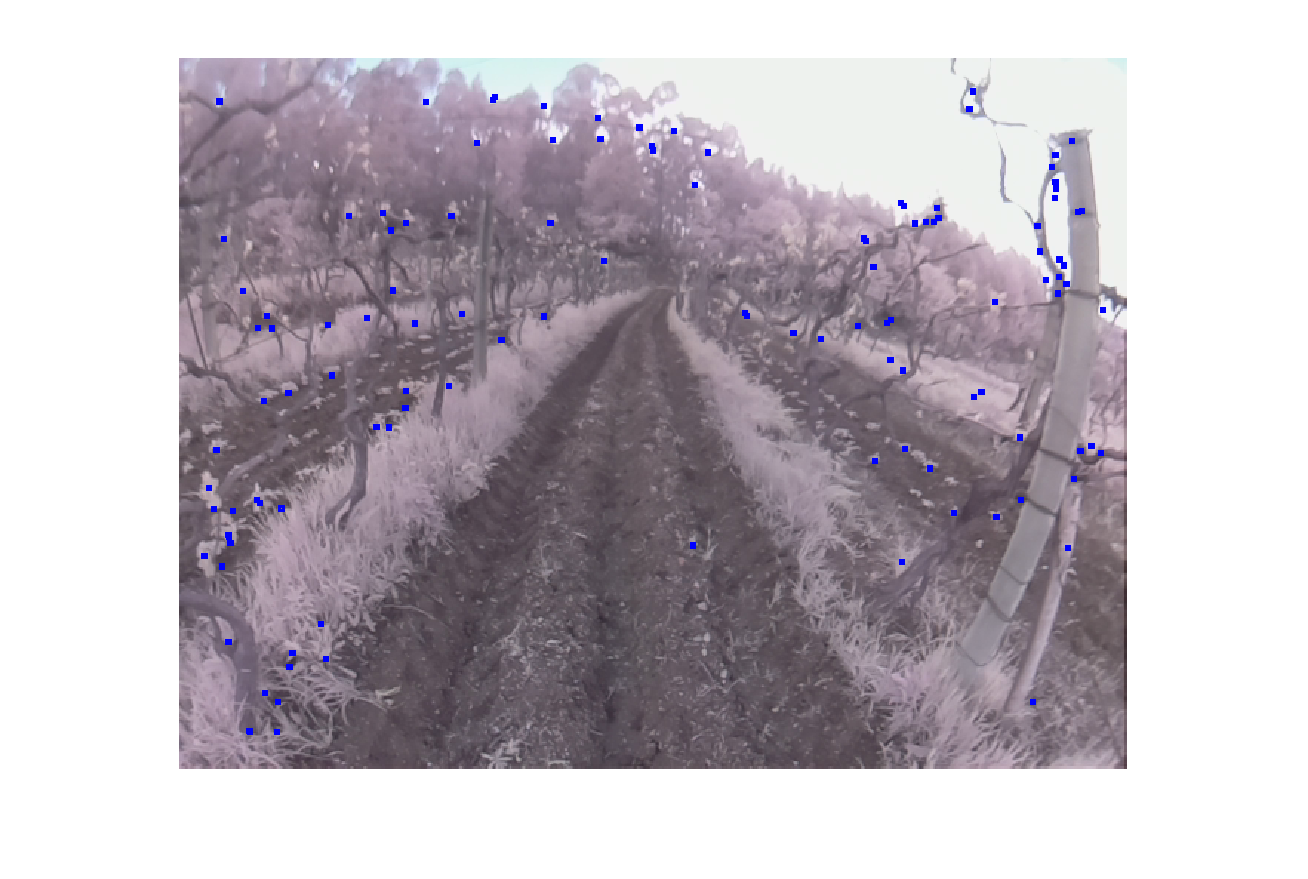
\includegraphics[width=0.4\textwidth]{metodosSURF.eps}}

	\subfloat[SIFT\label{fig:metodosSIFT}.]{
		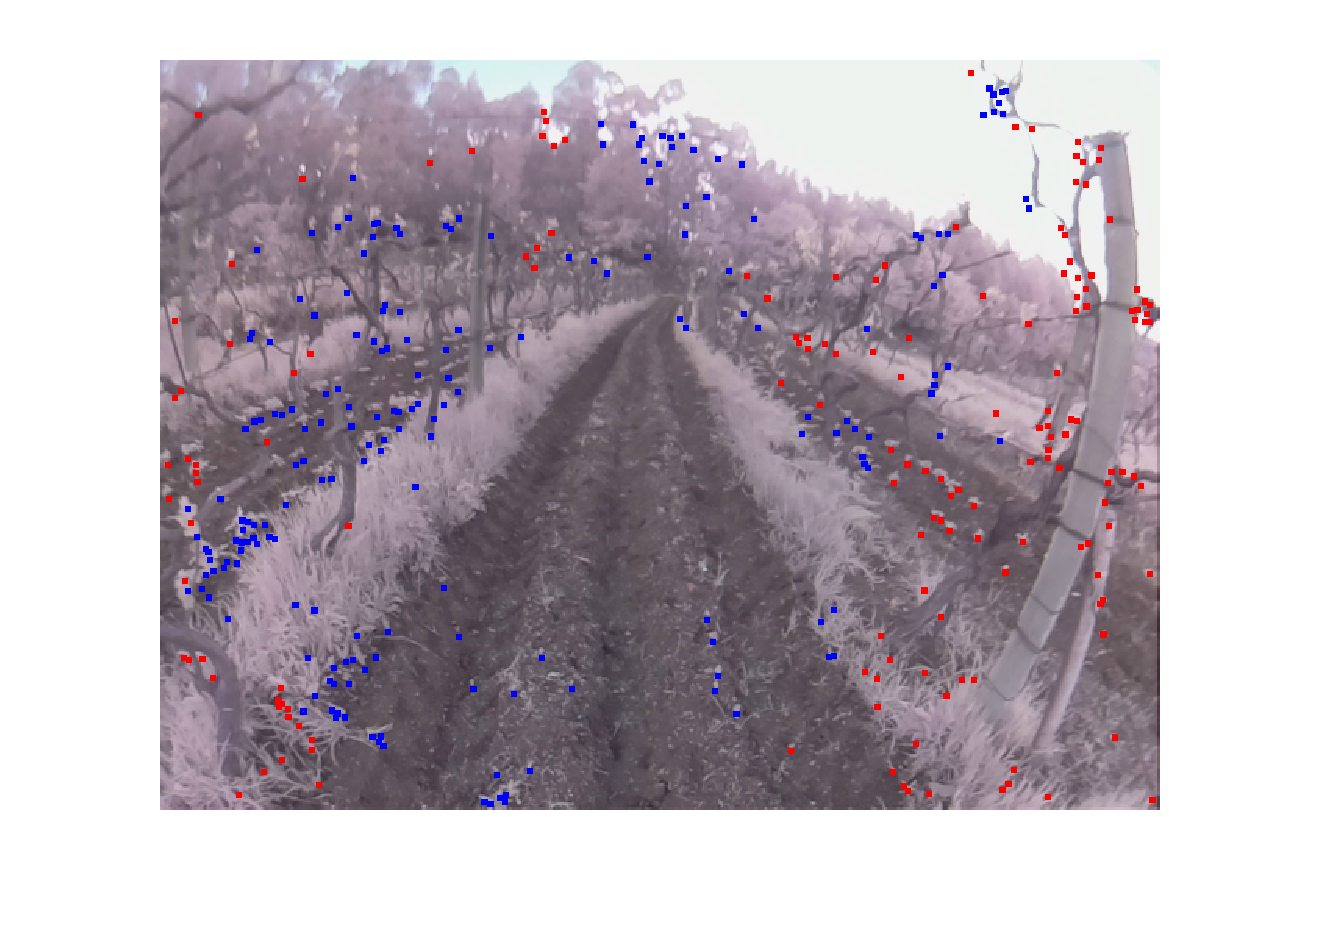
\includegraphics[width=0.4\textwidth]{metodosSIFT.eps}}
	\qquad
	\subfloat[HARRIS\label{fig:metodosHARRIS}.]{
		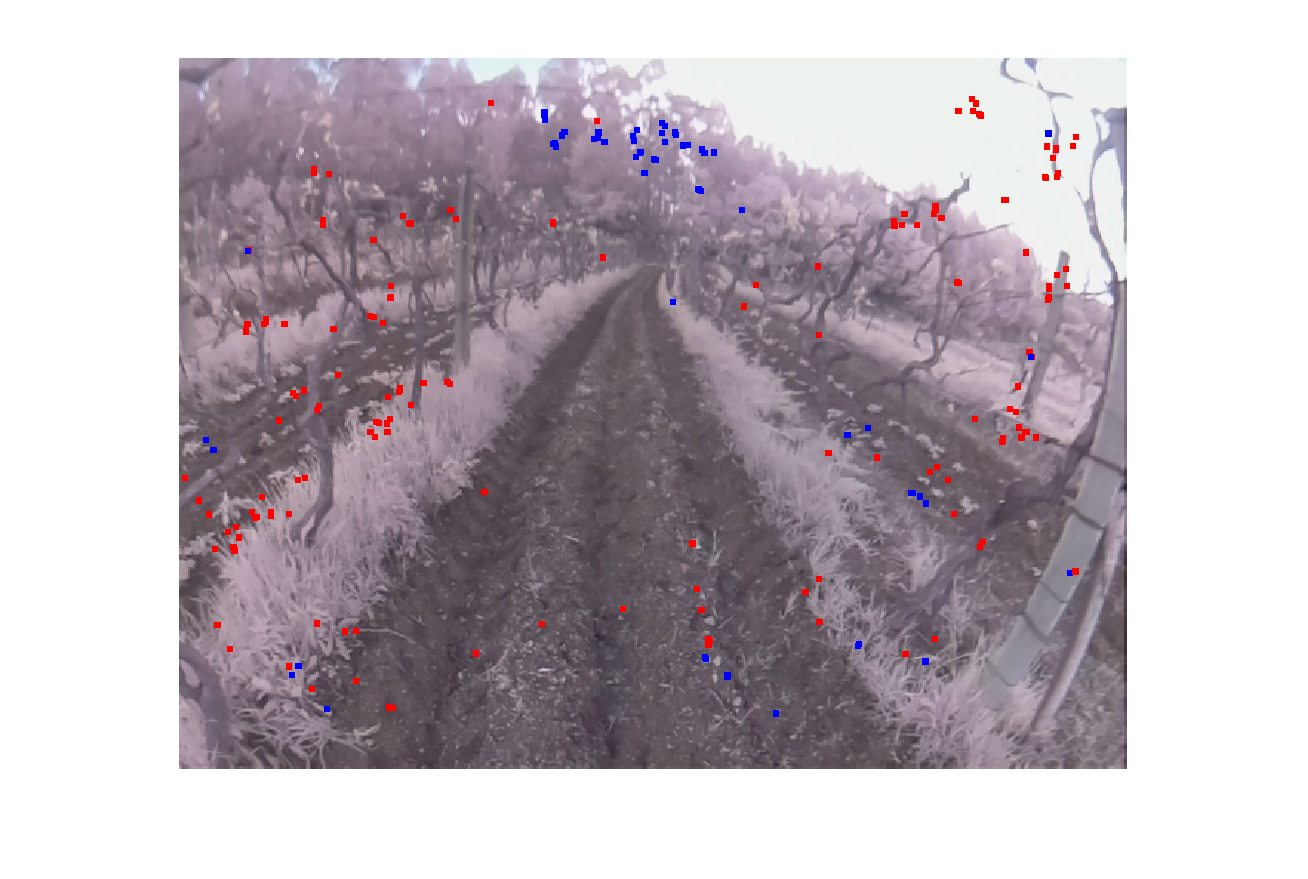
\includegraphics[width=0.4\textwidth]{metodosHARRIS.eps}}
	\caption{Distribuição dos pontos caracterisiticos para os quatro detetores des características}\label{fig:metodosALL}
\end{figure}


De notar que os pontos azuis são pontos de caracteristicas que têm correspondências corretas no próximo frame e os pontos vermelhos são \textit{outliers}, pontos com correspondência de caracteristicas erradas e/ou sem correspondências.

Os métodos têm as sua diferenças, desde logo a quantidade dos pontos com correspondência no frame seguinte. Desta forma, o método HARRIS é péssimo, devido às poucas correspondências, e o método SIFT discarta muitos pontos característicos de curta distância. A distribuição dos pontos caracteristicos é favoravél no método SURF , FAST e SIFT, sendo o primeiro o melhor, com maior seleção dos pontos na videiras, sendo estes mais estáveis e recomendados devido ao ambiente vinicula. Em termos de quantidade de pontos o método SIFT têm demasiados o que implica em maior tempo de processamento e maior número de frames perdidos entre processamento. Esta quantidade podia ser diminuida mas em cenários 
mais precários o algoritmo fica sujeito a encontrar um numero reduzido de pontos caracteristicos que impossibilitem o fucnionamento do algortimo. 

Assim, o método HARRIS é o pior devido a fraca qualidade e distribuição dos pontos caracteristicos. O método SIFT tem um grande tempo de processamento que caso a velocidade do robô seja baixa é uma solução plausivel devido a boa quantidade de pontos caracteristicos e boa distribuição. Por fim, o método FAST e SURF são os mais indicativos. Sendo, o último com melhor distribuição  dos pontos caracteristicos. 


\section{Comparação das combinações}


Como explicito no capítulo ~\ref{chap:odometria visual}, existem vários detetores de caracteristicas, descritores de caracteristicas e métodos de associação de caracteristicas. Desta forma, nesta dissertação são usados 4 detetores de caracteristicas, FAST, HARRIS, SIFT e SURF, 3 descritores de caracteristica, ORB, SIFT e SURF e 2 métodos de associação de caracteristicas, FLANN e Brute-Force, totalizando 24 combinações.

Os métodos são comparados pelos critérios :
\begin{itemize}
	\item \textbf{Imagens} - numero de imagens \ \textit{frames} processadas.
	\item \textbf{Tempo} - minimo, máximo e média de tempo nos ciclos de processamento.
	\item \textbf{Imagens perdidas (\textit{Lost Frames})} - quantidade de imagens perdidas(não analisadas) entre ciclos de processamento.
	\item \textbf{Número de pontos caracteristicos} - quantidade minima, máxima e média de pontos caracteristicos nos ciclos de processamento.
\end{itemize}


De forma a obter resultados coerentes é utilizado sempre a mesma movimentação, ficheiro \textit{bag}, em todos os teste. 


%\begin{figure}[h!] %colocar figura a seguir ao texto anterior
%	\begin{center}
%		\leavevmode		
%		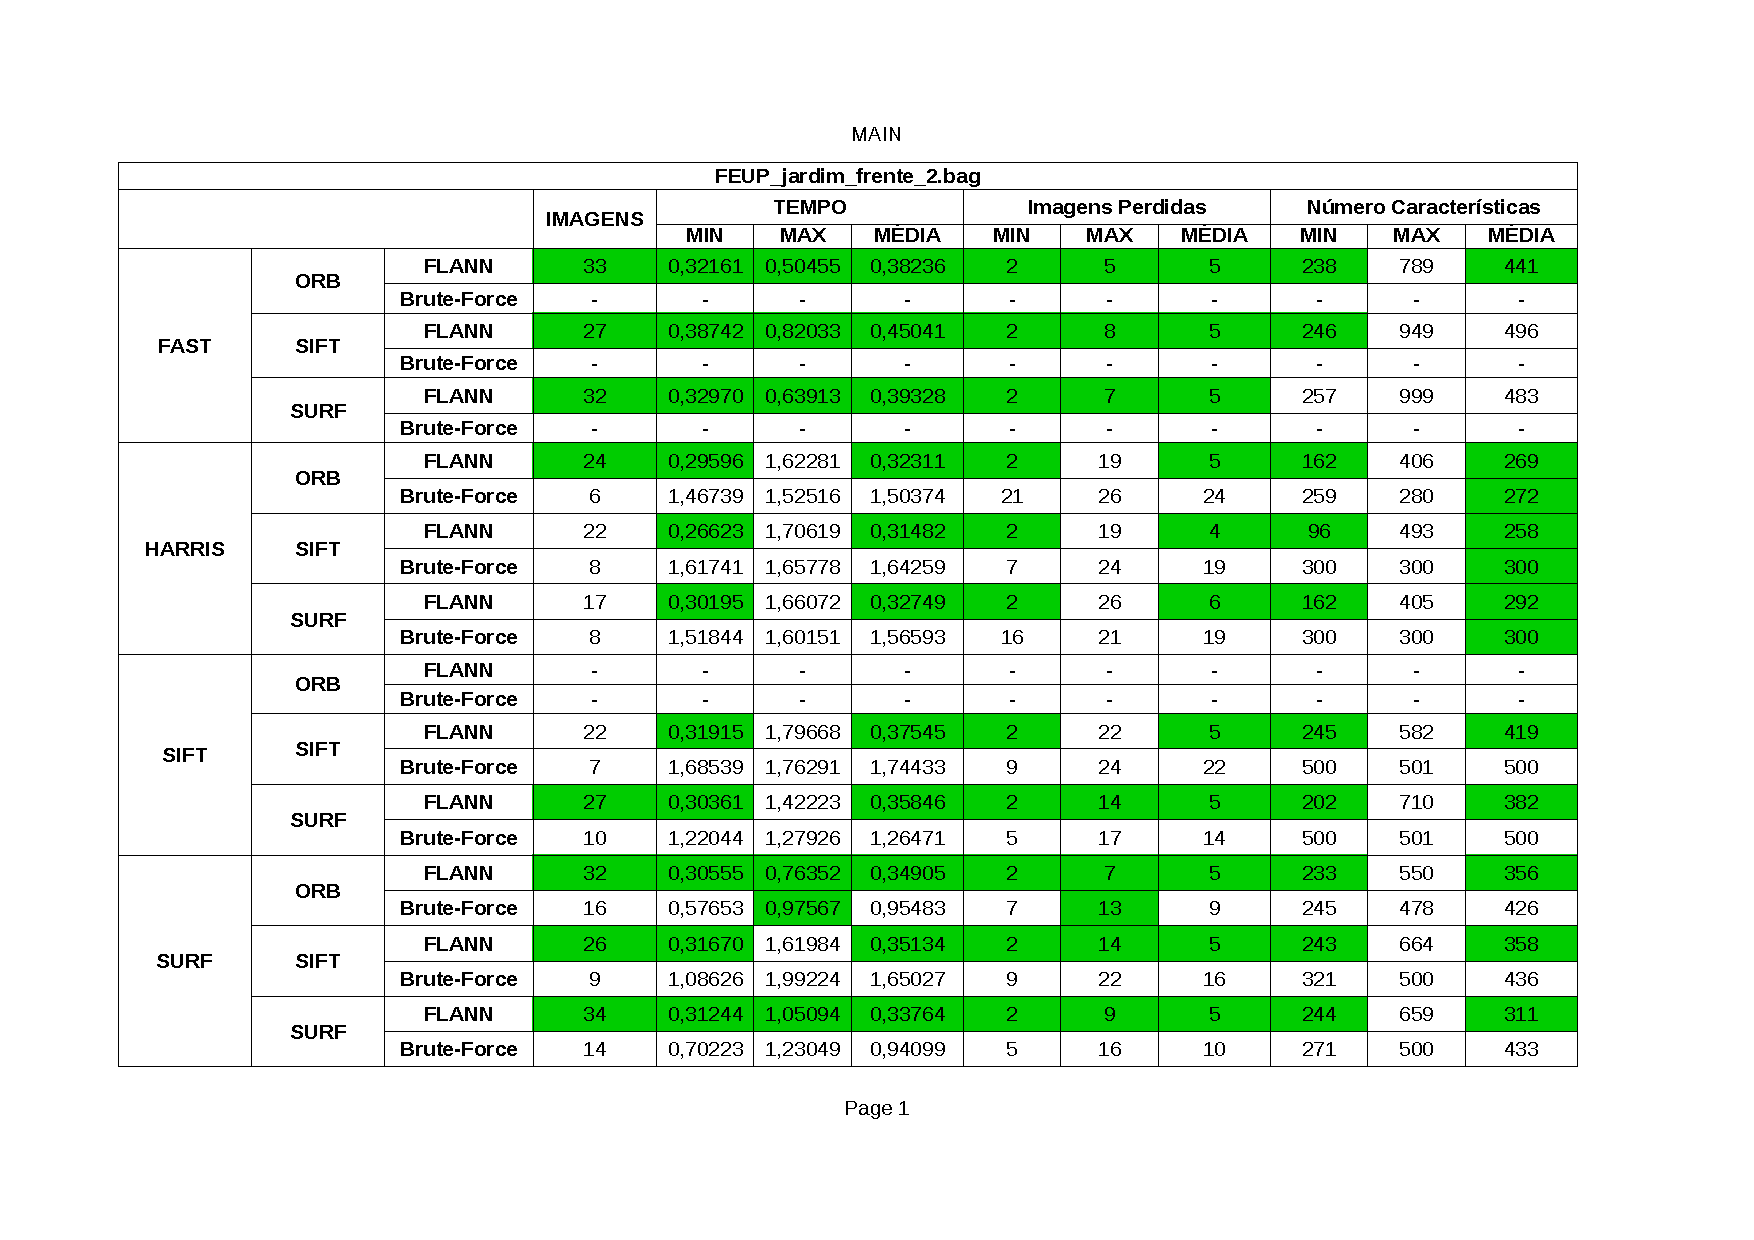
\includegraphics[width=1\textwidth]{compararMetodos.pdf}
%		\caption{Tabela de comparação das combinações dos métodos.}
%		\label{fig:compMet}
%	\end{center}
%\end{figure}


% Please add the following required packages to your document preamble:
% \usepackage{multirow}
% \usepackage[table,xcdraw]{xcolor}
% If you use beamer only pass "xcolor=table" option, i.e. \documentclass[xcolor=table]{beamer}
\begin{table}[h!]
	\centering
	\caption{Tabela de comparação das combinações dos métodos.}
	\label{tab:compMet}
	\resizebox{\textwidth}{!}{\begin{tabular}{|c|c|c|c|c|c|c|c|c|c|c|c|c|}
				\hline
				\multicolumn{13}{|c|}{FEUP\_jardim\_frente\_2.bag}                                                                                                                                                                                                                                                                                                        \\ \hline
				\multicolumn{3}{|c|}{}                                          &                            & \multicolumn{3}{c|}{TEMPO}                                                                          & \multicolumn{3}{c|}{IMAGENS PERDIDAS}                                              & \multicolumn{3}{c|}{NÚMERO CARACTERÍSTICAS}                     \\ \cline{5-13} 
				\multicolumn{3}{|c|}{\multirow{-2}{*}{}}                        & \multirow{-2}{*}{IMAGENS}  & MIN                             & MAX                             & MÉDIA                           & MIN                       & MAX                        & MÉDIA                     & MIN                         & MAX & MÉDIA                       \\ \hline
				&                        & FLANN       & \cellcolor[HTML]{32CB00}33 & \cellcolor[HTML]{32CB00}0,32161 & \cellcolor[HTML]{32CB00}0,50455 & \cellcolor[HTML]{32CB00}0,38236 & \cellcolor[HTML]{32CB00}2 & \cellcolor[HTML]{32CB00}5  & \cellcolor[HTML]{32CB00}5 & \cellcolor[HTML]{32CB00}238 & 789 & \cellcolor[HTML]{32CB00}441 \\ \cline{3-13} 
				& \multirow{-2}{*}{ORB}  & Brute-Force & -                          & -                               & -                               & -                               & -                         & -                          & -                         & -                           & -   & -                           \\ \cline{2-13} 
				&                        & FLANN       & \cellcolor[HTML]{32CB00}27 & \cellcolor[HTML]{32CB00}0,38742 & \cellcolor[HTML]{32CB00}0,82033 & \cellcolor[HTML]{32CB00}0,45041 & \cellcolor[HTML]{32CB00}2 & \cellcolor[HTML]{32CB00}8  & \cellcolor[HTML]{32CB00}5 & \cellcolor[HTML]{32CB00}246 & 949 & 496                         \\ \cline{3-13} 
				& \multirow{-2}{*}{SIFT} & Brute-Force & -                          & -                               & -                               & -                               & -                         & -                          & -                         & -                           & -   & -                           \\ \cline{2-13} 
				&                        & FLANN       & \cellcolor[HTML]{32CB00}32 & \cellcolor[HTML]{32CB00}0,32970 & \cellcolor[HTML]{32CB00}0,63913 & \cellcolor[HTML]{32CB00}0,39328 & \cellcolor[HTML]{32CB00}2 & \cellcolor[HTML]{32CB00}7  & \cellcolor[HTML]{32CB00}5 & 257                         & 999 & 483                         \\ \cline{3-13} 
				\multirow{-6}{*}{FAST}   & \multirow{-2}{*}{SURF} & Brute-Force & -                          & -                               & -                               & -                               & -                         & -                          & -                         & -                           & -   & -                           \\ \hline
				&                        & FLANN       & \cellcolor[HTML]{32CB00}24 & \cellcolor[HTML]{32CB00}0,29596 & 1,62281                         & \cellcolor[HTML]{32CB00}0,32311 & \cellcolor[HTML]{32CB00}2 & 19                         & \cellcolor[HTML]{32CB00}5 & \cellcolor[HTML]{32CB00}162 & 406 & \cellcolor[HTML]{32CB00}269 \\ \cline{3-13} 
				& \multirow{-2}{*}{ORB}  & Brute-Force & 6                          & 1,46739                         & 1,52516                         & 1,50374                         & 21                        & 26                         & 24                        & 259                         & 280 & \cellcolor[HTML]{32CB00}272 \\ \cline{2-13} 
				&                        & FLANN       & 22                         & \cellcolor[HTML]{32CB00}0,26623 & 1,70619                         & \cellcolor[HTML]{32CB00}0,31482 & \cellcolor[HTML]{32CB00}2 & 19                         & \cellcolor[HTML]{32CB00}4 & \cellcolor[HTML]{32CB00}96  & 493 & \cellcolor[HTML]{32CB00}258 \\ \cline{3-13} 
				& \multirow{-2}{*}{SIFT} & Brute-Force & 8                          & 1,61741                         & 1,65778                         & 1,64259                         & 7                         & 24                         & 19                        & 300                         & 300 & \cellcolor[HTML]{32CB00}300 \\ \cline{2-13} 
				&                        & FLANN       & 17                         & \cellcolor[HTML]{32CB00}0,30195 & 1,66072                         & \cellcolor[HTML]{32CB00}0,32749 & \cellcolor[HTML]{32CB00}2 & 26                         & \cellcolor[HTML]{32CB00}6 & \cellcolor[HTML]{32CB00}162 & 405 & \cellcolor[HTML]{32CB00}292 \\ \cline{3-13} 
				\multirow{-6}{*}{HARRIS} & \multirow{-2}{*}{SURF} & Brute-Force & 8                          & 1,51844                         & 1,60151                         & 1,56593                         & 16                        & 21                         & 19                        & 300                         & 300 & \cellcolor[HTML]{32CB00}300 \\ \hline
				&                        & FLANN       & -                          & -                               & -                               & -                               & -                         & -                          & -                         & -                           & -   & -                           \\ \cline{3-13} 
				& \multirow{-2}{*}{ORB}  & Brute-Force & -                          & -                               & -                               & -                               & -                         & -                          & -                         & -                           & -   & -                           \\ \cline{2-13} 
				&                        & FLANN       & 22                         & \cellcolor[HTML]{32CB00}0,31915 & 1,79668                         & \cellcolor[HTML]{32CB00}0,37545 & \cellcolor[HTML]{32CB00}2 & 22                         & \cellcolor[HTML]{32CB00}5 & \cellcolor[HTML]{32CB00}245 & 582 & \cellcolor[HTML]{32CB00}419 \\ \cline{3-13} 
				& \multirow{-2}{*}{SIFT} & Brute-Force & 7                          & 1,68539                         & 1,76291                         & 1,74433                         & 9                         & 24                         & 22                        & 500                         & 501 & 500                         \\ \cline{2-13} 
				&                        & FLANN       & \cellcolor[HTML]{32CB00}27 & \cellcolor[HTML]{32CB00}0,30361 & 1,42223                         & \cellcolor[HTML]{32CB00}0,35846 & \cellcolor[HTML]{32CB00}2 & \cellcolor[HTML]{32CB00}14 & \cellcolor[HTML]{32CB00}5 & \cellcolor[HTML]{32CB00}202 & 710 & \cellcolor[HTML]{32CB00}382 \\ \cline{3-13} 
				\multirow{-6}{*}{SIFT}   & \multirow{-2}{*}{SURF} & Brute-Force & 10                         & 1,22044                         & 1,27926                         & 1,26471                         & 5                         & 17                         & 14                        & 500                         & 501 & 500                         \\ \hline
				&                        & FLANN       & \cellcolor[HTML]{32CB00}32 & \cellcolor[HTML]{32CB00}0,30555 & \cellcolor[HTML]{32CB00}0,76352 & \cellcolor[HTML]{32CB00}0,34905 & \cellcolor[HTML]{32CB00}2 & \cellcolor[HTML]{32CB00}7  & \cellcolor[HTML]{32CB00}5 & \cellcolor[HTML]{32CB00}233 & 550 & \cellcolor[HTML]{32CB00}356 \\ \cline{3-13} 
				& \multirow{-2}{*}{ORB}  & Brute-Force & 16                         & 0,57653                         & \cellcolor[HTML]{32CB00}0,97567 & 0,95483                         & 7                         & \cellcolor[HTML]{32CB00}13 & 9                         & 245                         & 478 & 426                         \\ \cline{2-13} 
				&                        & FLANN       & \cellcolor[HTML]{32CB00}26 & \cellcolor[HTML]{32CB00}0,31670 & 1,61984                         & \cellcolor[HTML]{32CB00}0,35134 & \cellcolor[HTML]{32CB00}2 & \cellcolor[HTML]{32CB00}14 & \cellcolor[HTML]{32CB00}5 & \cellcolor[HTML]{32CB00}243 & 664 & \cellcolor[HTML]{32CB00}358 \\ \cline{3-13} 
				& \multirow{-2}{*}{SIFT} & Brute-Force & 9                          & 1,08626                         & 1,99224                         & 1,65027                         & 9                         & 22                         & 16                        & 321                         & 500 & 436                         \\ \cline{2-13} 
				&                        & FLANN       & \cellcolor[HTML]{32CB00}34 & \cellcolor[HTML]{32CB00}0,31244 & \cellcolor[HTML]{32CB00}1,05094 & \cellcolor[HTML]{32CB00}0,33764 & \cellcolor[HTML]{32CB00}2 & \cellcolor[HTML]{32CB00}9  & \cellcolor[HTML]{32CB00}5 & \cellcolor[HTML]{32CB00}244 & 659 & \cellcolor[HTML]{32CB00}311 \\ \cline{3-13} 
				\multirow{-6}{*}{SURF}   & \multirow{-2}{*}{SURF} & Brute-Force & 14                         & 0,70223                         & 1,23049                         & 0,94099                         & 5                         & 16                         & 10                        & 271                         & 500 & 433                         \\ \hline
		\end{tabular}}
\end{table}



A tabela ~\ref{tab:compMet} ilustra os resultados obtidos nos testes. As combinações em que  o algoritmo resulta em erro por baixo número de pontos caracteristicos e / ou baixa quantidade de associação de pontos caracteristicos durante uma grande quantidade de ciclos de processamento é representada pelo simbolo \textbf{-}. De forma a melhor intrepertação da tabela os valores com bons resultados estão coloridos de verde. 

Assim, na coluna \textbf{Imagens} a maior quantidade analisadas no algoritmo melhor. Nas colunas \textbf{minimos, máximo e médios do Tempo , Imagens Perdidas e numero de pontos caracteristicos} quanto menor o valor melhor os resultados. 

Analisando a tabela, as combinações com o simbolo \textbf{-} ou sem células coloridas a verde são péssimas soluções. Desta forma, a associação \textbf{Brute-Force} não têm nenhuma solução devido ao maior tempo de processamento em relação ao método \textbf{FLANN} e a menor coerência de correspondência de pontos caracteristicos. Assim, das restantes combinações, os detetores de \textbf{HARRIS} e \textbf{SIFT} têm algumas soluções possiveis de utilizar mas com parâmetros fracos, tais como a quantidade de Imagens, tempo máximo e máxima quantidade de imagens perdidas, tendo estes parâmetros absordamente maiores. Dos restantes métodos, sendo todos combinações razoaveís de implementar, é de realçar as combinações \textbf{FAST/ORB/FLANN} e \textbf{SURF/ORB/FLANN} com os melhores parâmetros, sendo as utilizadas nos restantes testes.






\section{Cinemática Agrov16}

A cinemática é a área da Física que estuda o movimento dos corpos. Em robótica móvel a cinemática estabelece relações entre o deslocamento (locomoção) do robô e a atuação a ele imposta.

A cinemática direta estabelece modelos que estimam o deslocamento do robô dada uma atuação, por exemplo, velocidades imposta às suas rodas. 

A cinemática reversa estabelece modelos que estimam a atuação necessária para que o robô realize o determinado deslocamento, por exemplo, percorrer uma trajetória.

Comumente, os modelos cinemáticos são baseados em equações diferenciais de primeira ordem não lineares. Tais modelos são linearizados e discretizados no tempo quanto utilizados em aplicações robótica.


O modelo não leva em conta a inércia do robô, deformações em sua estrutura, forças oriundas do deslocamento (atrito, escorregamento, etc.), e demais fatores internos e externos que possam agetar a locomoção.


O robô AgrobV16, figura ~\ref{fig:agrobv16}, possui 4 rodas com tração mas, a cinemática no centro de massa é equivalente à cinemática de tração diferencial. 

\begin{figure}[h!] %colocar figura a seguir ao texto anterior
	\begin{center}
		\leavevmode		
		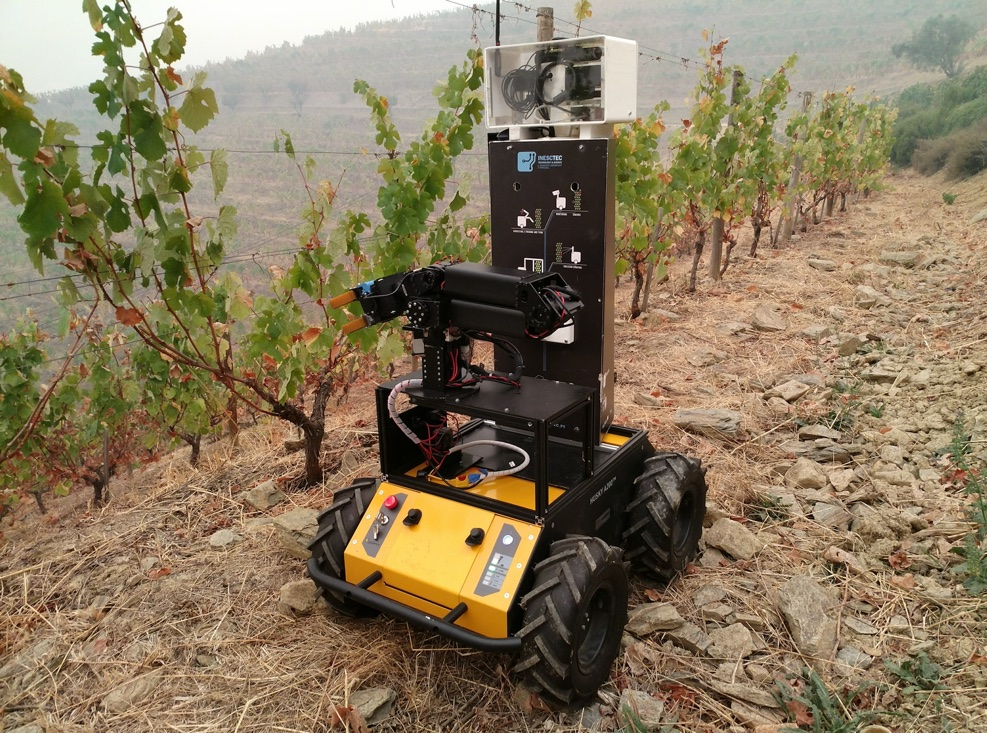
\includegraphics[width=0.6\textwidth]{agrobv16.jpg}
		\caption{Robô AgrobV16.}
		\label{fig:agrobv16}
	\end{center}
\end{figure}


Desta forma, um robô diferencial possui 2 rodas com tração independentes e um ou mais pontos de contacto usualmente proporcionados por rodas sem tração, no caso do AgrobV16 possui 4 rodas de tração mas a tração é aos pares resultando na equivalência de 2 rodas de tração.

A única forma de atuação em um robô diferencial é pela imposição de velocidades independentes em cada roda. O robô diferencial possui estabilidade estática mas não é um robô omnidirecional dado que é incapaz de se deslocar sobre o seu eixo transversal. Como ilustrado na figura ~\ref{fig:kinematicAgrob} , o centro de rotação do robô está localizado na intersecção dos eixos transversal (\textbf{$Y_R$}) e longitudinal (\textbf{$X_R$}).

\begin{figure}[h!] %colocar figura a seguir ao texto anterior
	\begin{center}
		\leavevmode		
		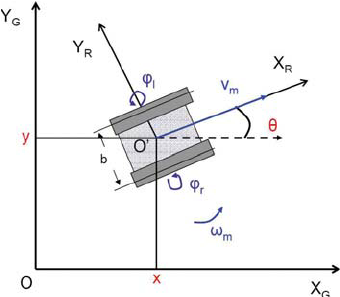
\includegraphics[width=0.6\textwidth]{kinematicAgrob.png}
		\caption{Modelo de Cinemática diferencial.}
		\label{fig:kinematicAgrob}
	\end{center}
\end{figure}

Considerando : 
\begin{itemize}
	\item \textbf{b} a distância entre rodas.
	\item \textbf{$\phi_r$} o raio da roda da direita.
	\item \textbf{$\phi_l$} o raio da roda da esquerda.
	\item \textbf{$v_r$} a velocidade da roda da direita.
	\item \textbf{$v_l$} a velocidade da roda da esquerda.
	\item \textbf{$v_m$} a velocidade linear do robô.
	\item \textbf{$w_m$} a velocidade angular do robô.
	\item $\textbf{$\theta$}$ o ângulo do robô , ângulo entre $v_m$ e eixo x.
\end{itemize}

Obtemos:
\[ \left\{\begin{array}{ccc}
	v_1(t) = v_m(t) cos( \theta(t))\\ 
	v_2(t) = v_m(t) sin( \theta(t))\\ 
	w(t) = w(t)
\end{array}\right. \]

Originando: 

\[ v(t) = \frac{v_1(t)+v_2(t)}{2} \]

\[  w(t) = \frac{v_1(t)-v_2(t)}{b} \]

Em tempo discreto :

\[ d(i) = \frac{d_1(t)+d_2(t)}{2} \]

\[ \Delta \theta (i) = \frac{d_1(t)-d_2(t)}{b} \]

Sendo a posição seguinte dependente da posição atual mais o deslocamento do robô em relação à velocidade resulta:

\[ \left\{\begin{array}{ccc}
x(i+1) = x(i) + d(i) cos( \theta(i) + \frac{\Delta \theta(i)}{2})\\ 
y(i+1) = y(i) + d(i) sin( \theta(i) + \frac{\Delta \theta(i)}{2})\\ 
\theta (i+1) = \theta (i) + \Delta \theta (i)
\end{array}\right. \]


\section{Testes}

De forma a validar o algoritmo de localização os testes requerem a quantificação do erro. O erro é descrito com a diferença entre o valor real e o valor medido.

As coordenadas reais têm de ser obtidas através de um sensor externo, tal como a laser baseado em localização, odometria das rodas ou mesmo uma fita métrica. Desta forma, os testes são realizados no robô AgrobV16 e as coordenadas reais são obtidas através da odometria das rodas, tópico \textbf{husky...}. 


Os percursos efetuados foram : estático, movimento em linha reta, movimento em L (semi-quadrado) e percurso quadrangular. De notar que os percursos foram realizados com velocidades baixas. Assim, a câmara consegue extrair um maior número de características e por consequência o erro da trajetória estimada será menor.  

